\documentclass[a4paper]{scrbook}
\usepackage[utf8]{inputenc}
\usepackage[ngerman]{babel}

\usepackage{array}            % Tabellen im Mathemodus (Matrizen)
\usepackage{graphicx}         % Einbindung von Grafiken
\usepackage{braket}           % ermöglicht die Verwendung von Diracs Bra-Ket-Notation
\usepackage{esdiff}           % für Ableitungen


\usepackage{hyperref}         % für automatische Verlinkungen in der pdf
\usepackage{datatool}	      % muss verwendet werden, da glossaries sonst einen Fehler verursacht
\usepackage[toc]{glossaries}  % Glossar

\makeglossaries
\makeindex

% Glossar
\newglossaryentry{OST}{name={OST}, description={Opposite Side Tagger}}
\newglossaryentry{Toy MC}{name={Toy MC}, description={Zur Validierung des Fitters werden zufällig Daten gemäß einer gewünschten Verteilung generiert und im Anschluss gefittet}}


% Definiere Kürzel
\newcommand{\SJPsi}{S_{J/\Psi K_s^0}}
\newcommand{\CP}{$\mathcal{CP}$}
\newcommand{\im}{\mathrm{i}}
\newcommand{\e}{\mathrm{e}}


\begin{document}

% Binde Titelseite ein
\begin{titlepage}
\begin{center}
 
\Large\textbf{Fakultät für Physik und Astronomie\\
Ruprecht-Karls-Universität Heidelberg}

\vspace{17cm}

\normalsize
Bachelorarbeit in Physik\\
eingereicht von\\
\vspace{0.5cm}
\Large\textbf{Patrick Fahner}\\
\normalsize
\vspace{0.5cm}
geboren in Mannheim (Deutschland)\\
\vspace{0.5cm}
\Large\textbf{August 2013}
\normalsize

\newpage




\Large\textbf{About ...}

\vspace{18cm}

\normalsize
This Bachelor Thesis has been carried out by XYZ at the\\
ABC Institute in Heidelberg\\
under the supervision of\\
Prof. Max Mustermann

\vfill
\end{center}

\end{titlepage}



\chapter{CP-Verletzung in B-Meson-Systemen}

\section{B-Mesonen und der Zerfallskanal \Decaychannel}
\subsection{Das Standardmodell der Teilchenphysik}
Im Standardmodell der Teilchenphysik gibt es 17 elementare Bausteine der Materie (siehe Abb. \ref{fig:standardmodell}): 12 Fermionen, davon 6 Quarks (u, d, c, s, t, b), die sich im engeren Sinne zur Materie hadronisieren oder Mesonen bilden, und 6 Leptonen (e, $\mathrm{\mu}$, $\mathrm{\tau}$ sowie die jweiligen Neutrinos $\mathrm{\nu_e}$, $\mathrm{\nu_{\mu}}$, $\mathrm{\nu_{\tau}}$). Von diesen 12 Fermionen existieren jeweils noch Antiteilchen (gleiche Eigenschaften, aber entgegengesetzte Masse). Das Standardmodell enthält weiterhin 4 Eichbosonen (Photon, Gluon, Z- und W$^{\pm}$-Boson), die die 3 der 4 elementaren Kräfte übertragen: die elektromagnetische, starke und schwache Wechselwirkung. Das für die Gravitation postulierte Graviton konnte bislang nicht nachgewiesen werden. Ergänzt wird das Standardmodell, durch das Higgs-Boson, welches als Teil des Higgs-Mechanismus den Elementarteilchen seine Masse verleiht und Gegenstand aktueller Forschung ist. Mit hoher Wahrscheinlichkeit gelang jüngst der Nachweis des Higgs am CERN \cite{higgs}.

\begin{figure}[hptb]
\centering
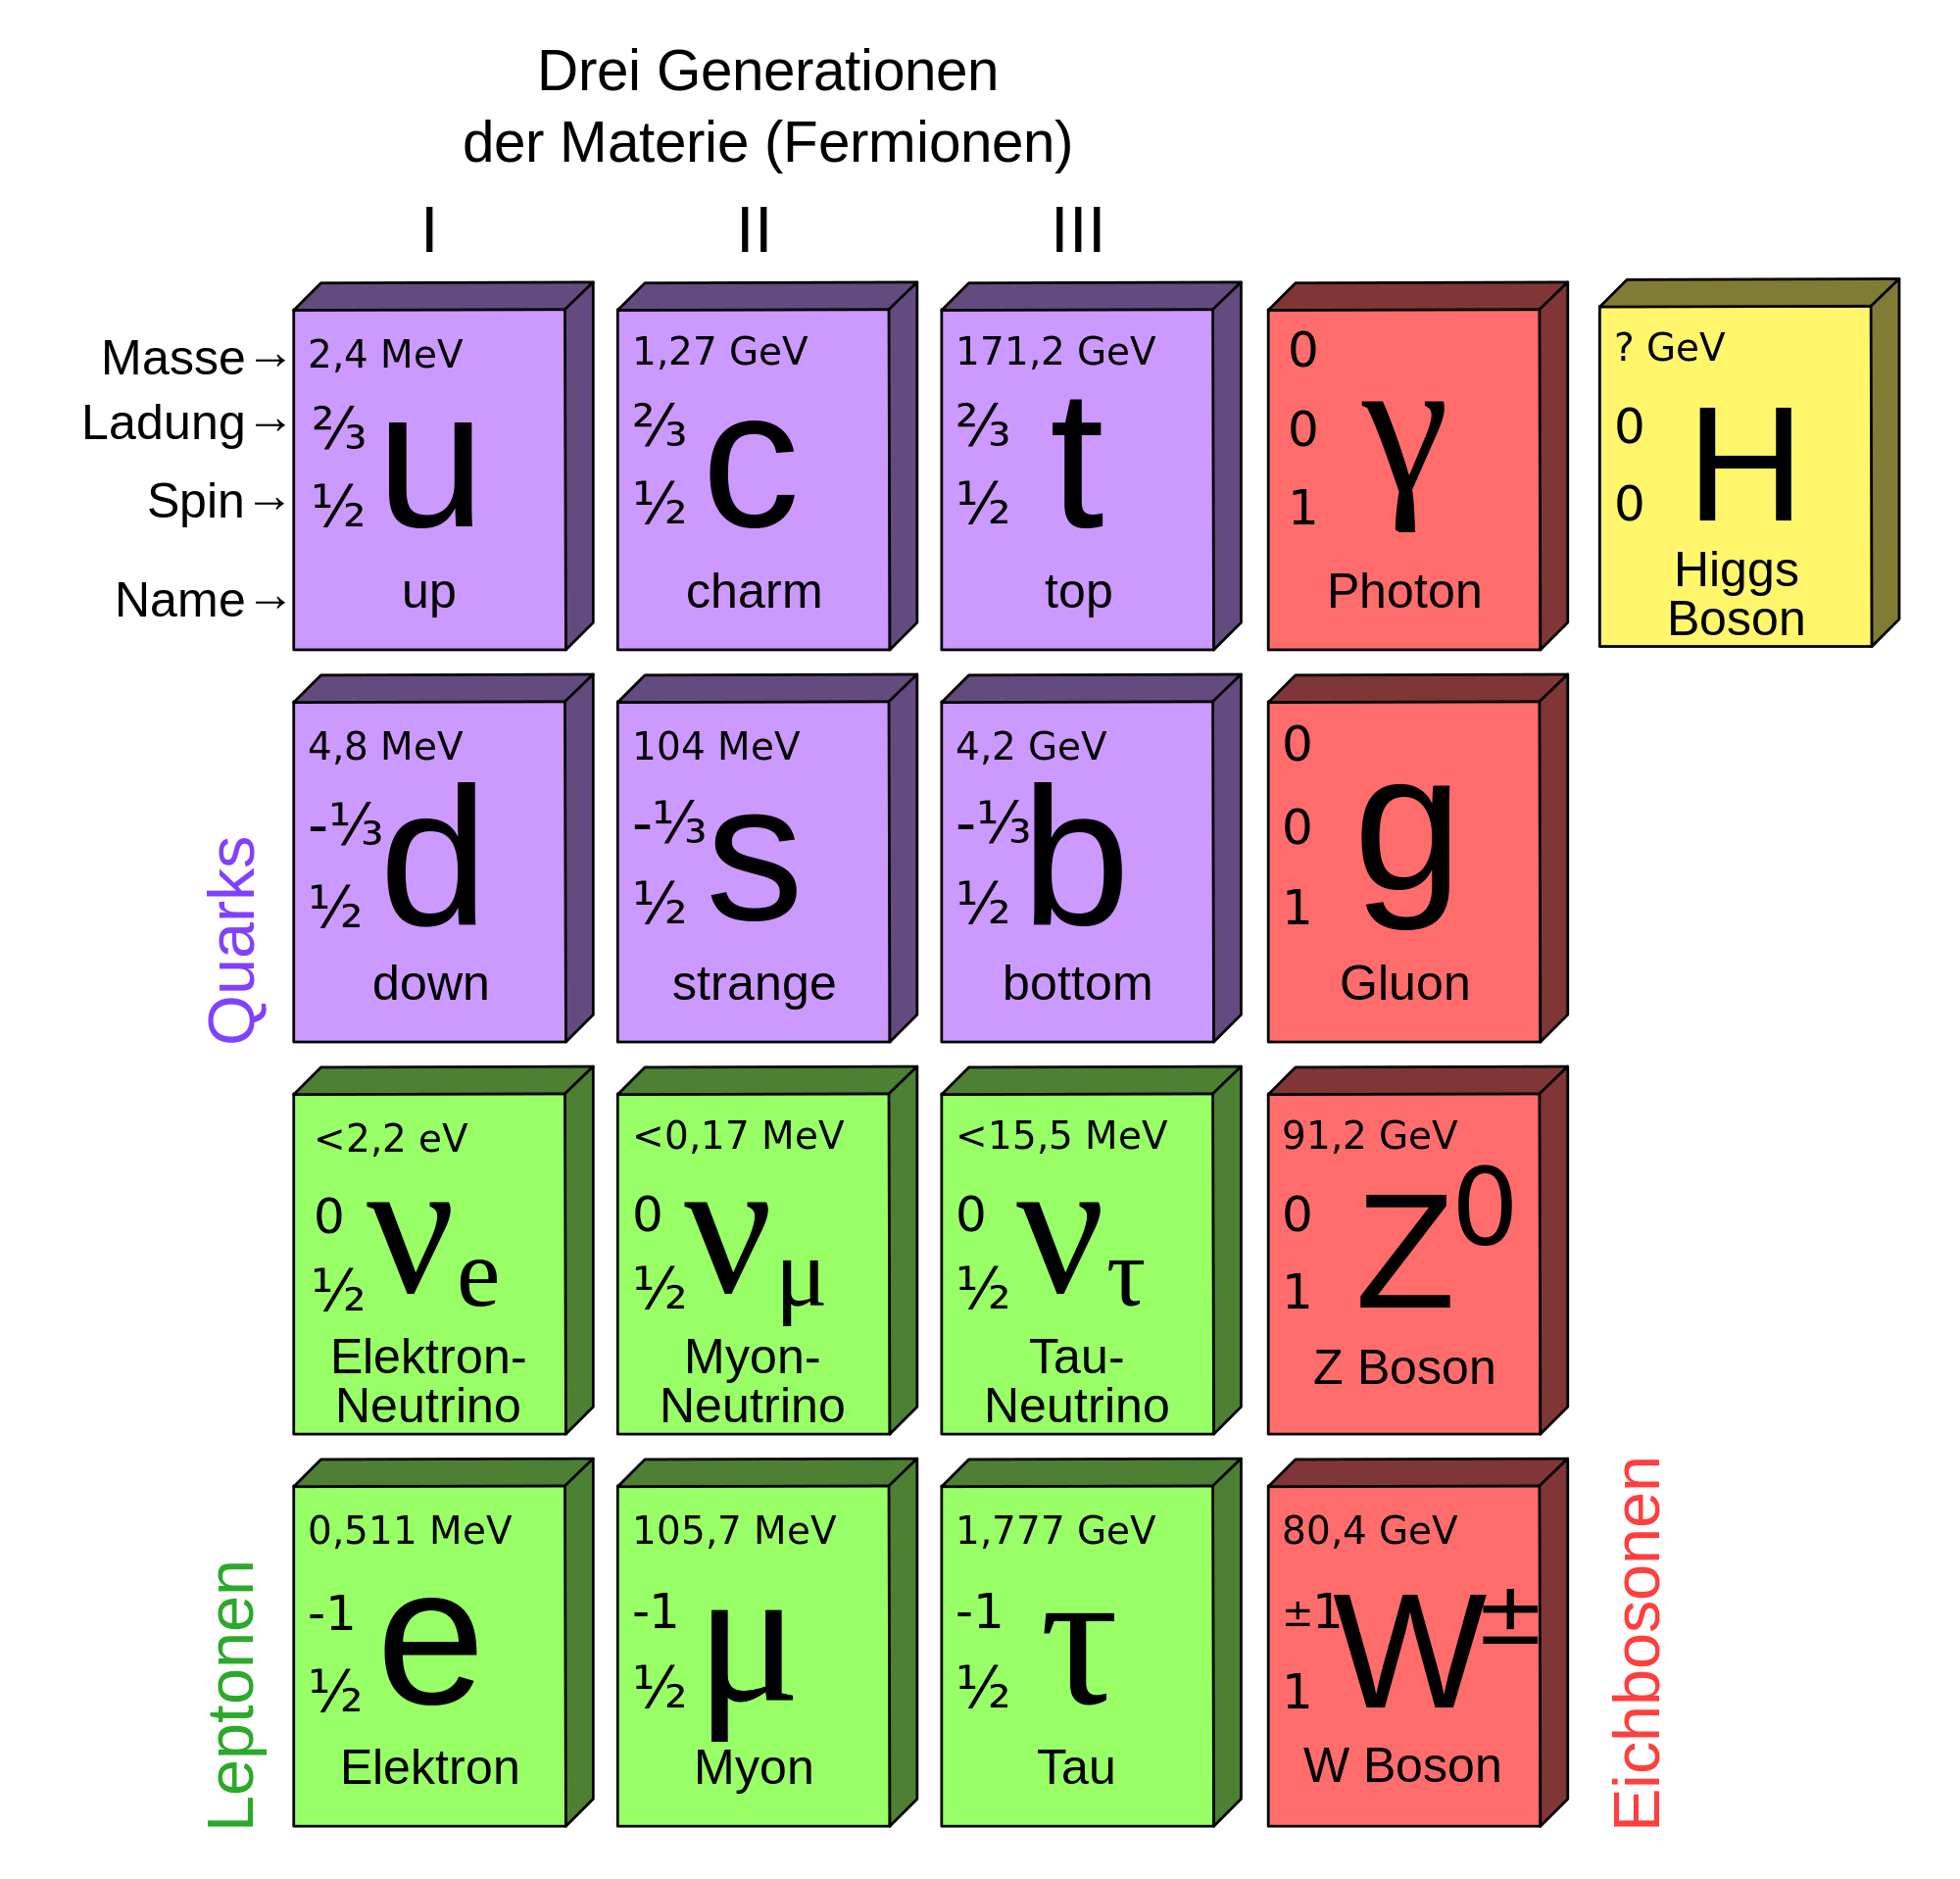
\includegraphics[width=0.5\textwidth]{standardmodell}
\caption{Das Standardmodell der Teilchenphysik \cite{wiki_standard}}
\label{fig:standardmodell}
\end{figure}

\subsection{B-Mesonen und ihre Mischung}
Mesonen sind Paare aus Quarks und Antiquarks beliebigen Flavours. B-Mesonen insbesondere bestehen aus einem Anti-b-Quark ($\mathrm{\overline{b}}$) mit einem u-, d-, c- oder s-Quark beziehungsweise aus der Kombination der jeweiligen Antiteilchen (Anti-B-Mesonen).

Die in dieser Arbeit betrachteten \Bd-Mesonen haben demnach die Quarkzusammensetzung $\Ket{\text{\Bd}} = \Ket{\overline{b}d}$ und sind elektrisch neutral. Solch neutrale Mesonen besitzen die Eigenschaft, dass sie sich in ihre Antiteilchen wandeln können und umgekehrt. Es findet folglich eine Oszillation zwischen \Bd und \Bdbar statt, die man auch Mischung nennt. Abbildung \ref{fig:bmixing} zeigt zwei mögliche Feynmangraphen für diesen Prozess. Innerhalb der Schleifen kann die Energieerhaltung kurzzeitig verletzt werden, sodass auch kurzerhand die deutlich schweren top-Quarks enstehen können. Zu diesem Mischungsprozess leisten sie sogar einen dominanten Beitrag. Präzise Messungen der \Bd-Mischung erlauben Aussagen bspw. über die top-Masse und grenzen damit das Standardmodell ein, gleichzeitig erhofft man sich, durch noch präzisere Messungen Hinweise auf \glqq neue Physik\grqq zu finden, die sich dann in kleinsten Korrekturen innerhalb der Schleife bemerkbar machen würden.

\begin{figure}[hptb]
\centering
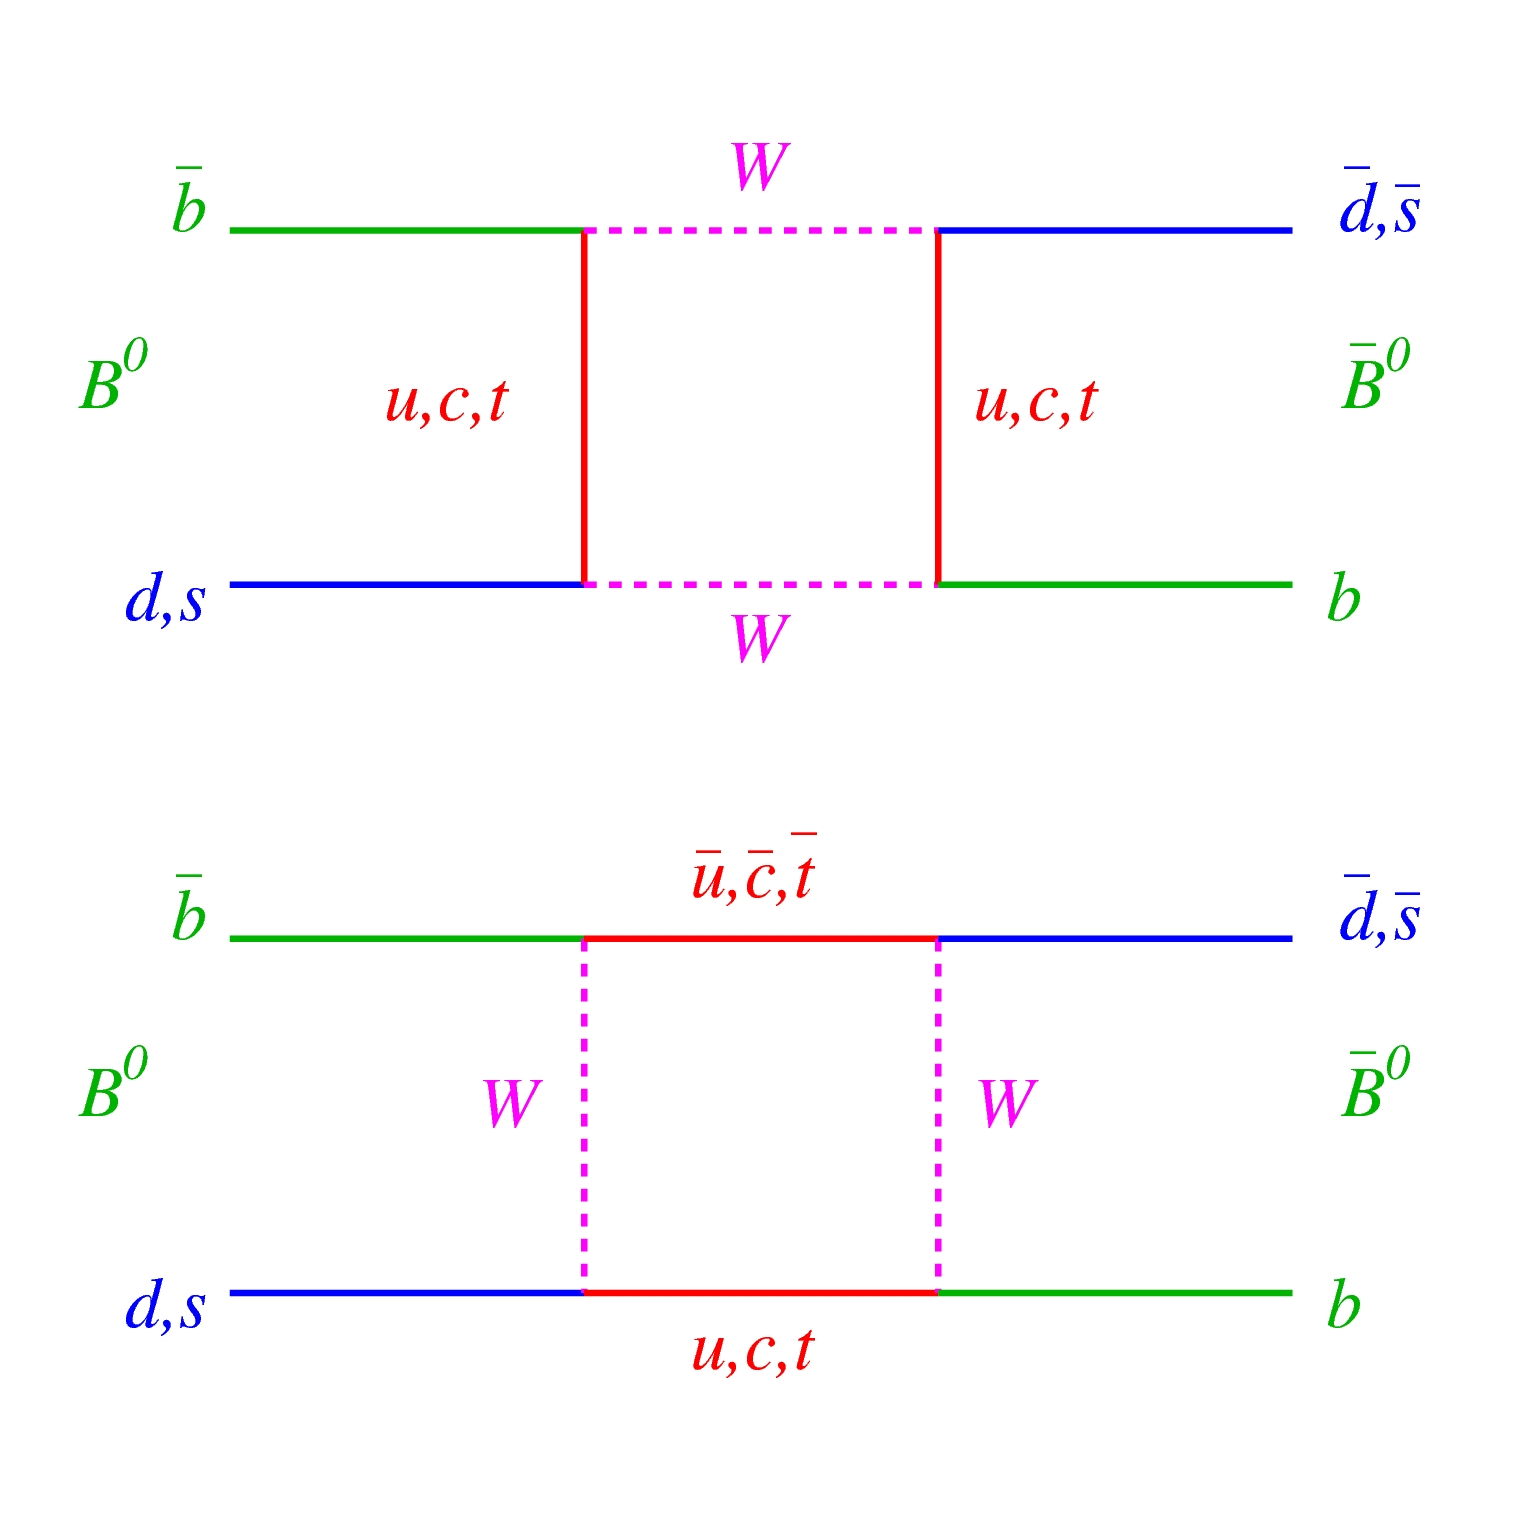
\includegraphics[width=0.5\textwidth]{bmixing}
\caption{Feynmangraphen zur Mischung von \Bd- und \Bdbar-Mesonen}
\label{fig:bmixing}
\end{figure}


\subsection{Der Zerfallskanal \Decaychannel}
In dieser Arbeit wird der Zerfallskanal \Decaychannel betrachtet. Abbildung \ref{fig:decay} zeigt entsprechende Feynmangraphen. Jener Kanal ist auch als \glqq goldener\grqq Zerfallskanal für die Messung der \CP-Verletzung bekannt. Hintergrund ist, dass der Endzustand $\Ket{\JPsi\Kshort}$ ein \CP-Eigenzustand ist ($\text{\CP}\Ket{\JPsi\Kshort} = - \Ket{\JPsi\Kshort}$). Die Teilchen $\JPsi$ und $\Kshort$ haben die Flavoureigenzustände $\Ket{\JPsi} = \Ket{c\overline{c}}$ sowie $\Ket{\Kshort} = \tfrac{1}{\sqrt{2}}\left(\Ket{d\overline{s}}-\Ket{s\overline{d}}\right)$. Diese Teilchen sind ebenfalls nicht stabil und zerfallen unter anderem weiter gemäß $\JPsi \rightarrow \mu^+\mu^-$ und $\Kshort \rightarrow \pi^+\pi^-$, was zur Rekonstruktion der \Bd-Mesonen im Detektor genutzt wird.

\begin{figure}[hptb]
\centering
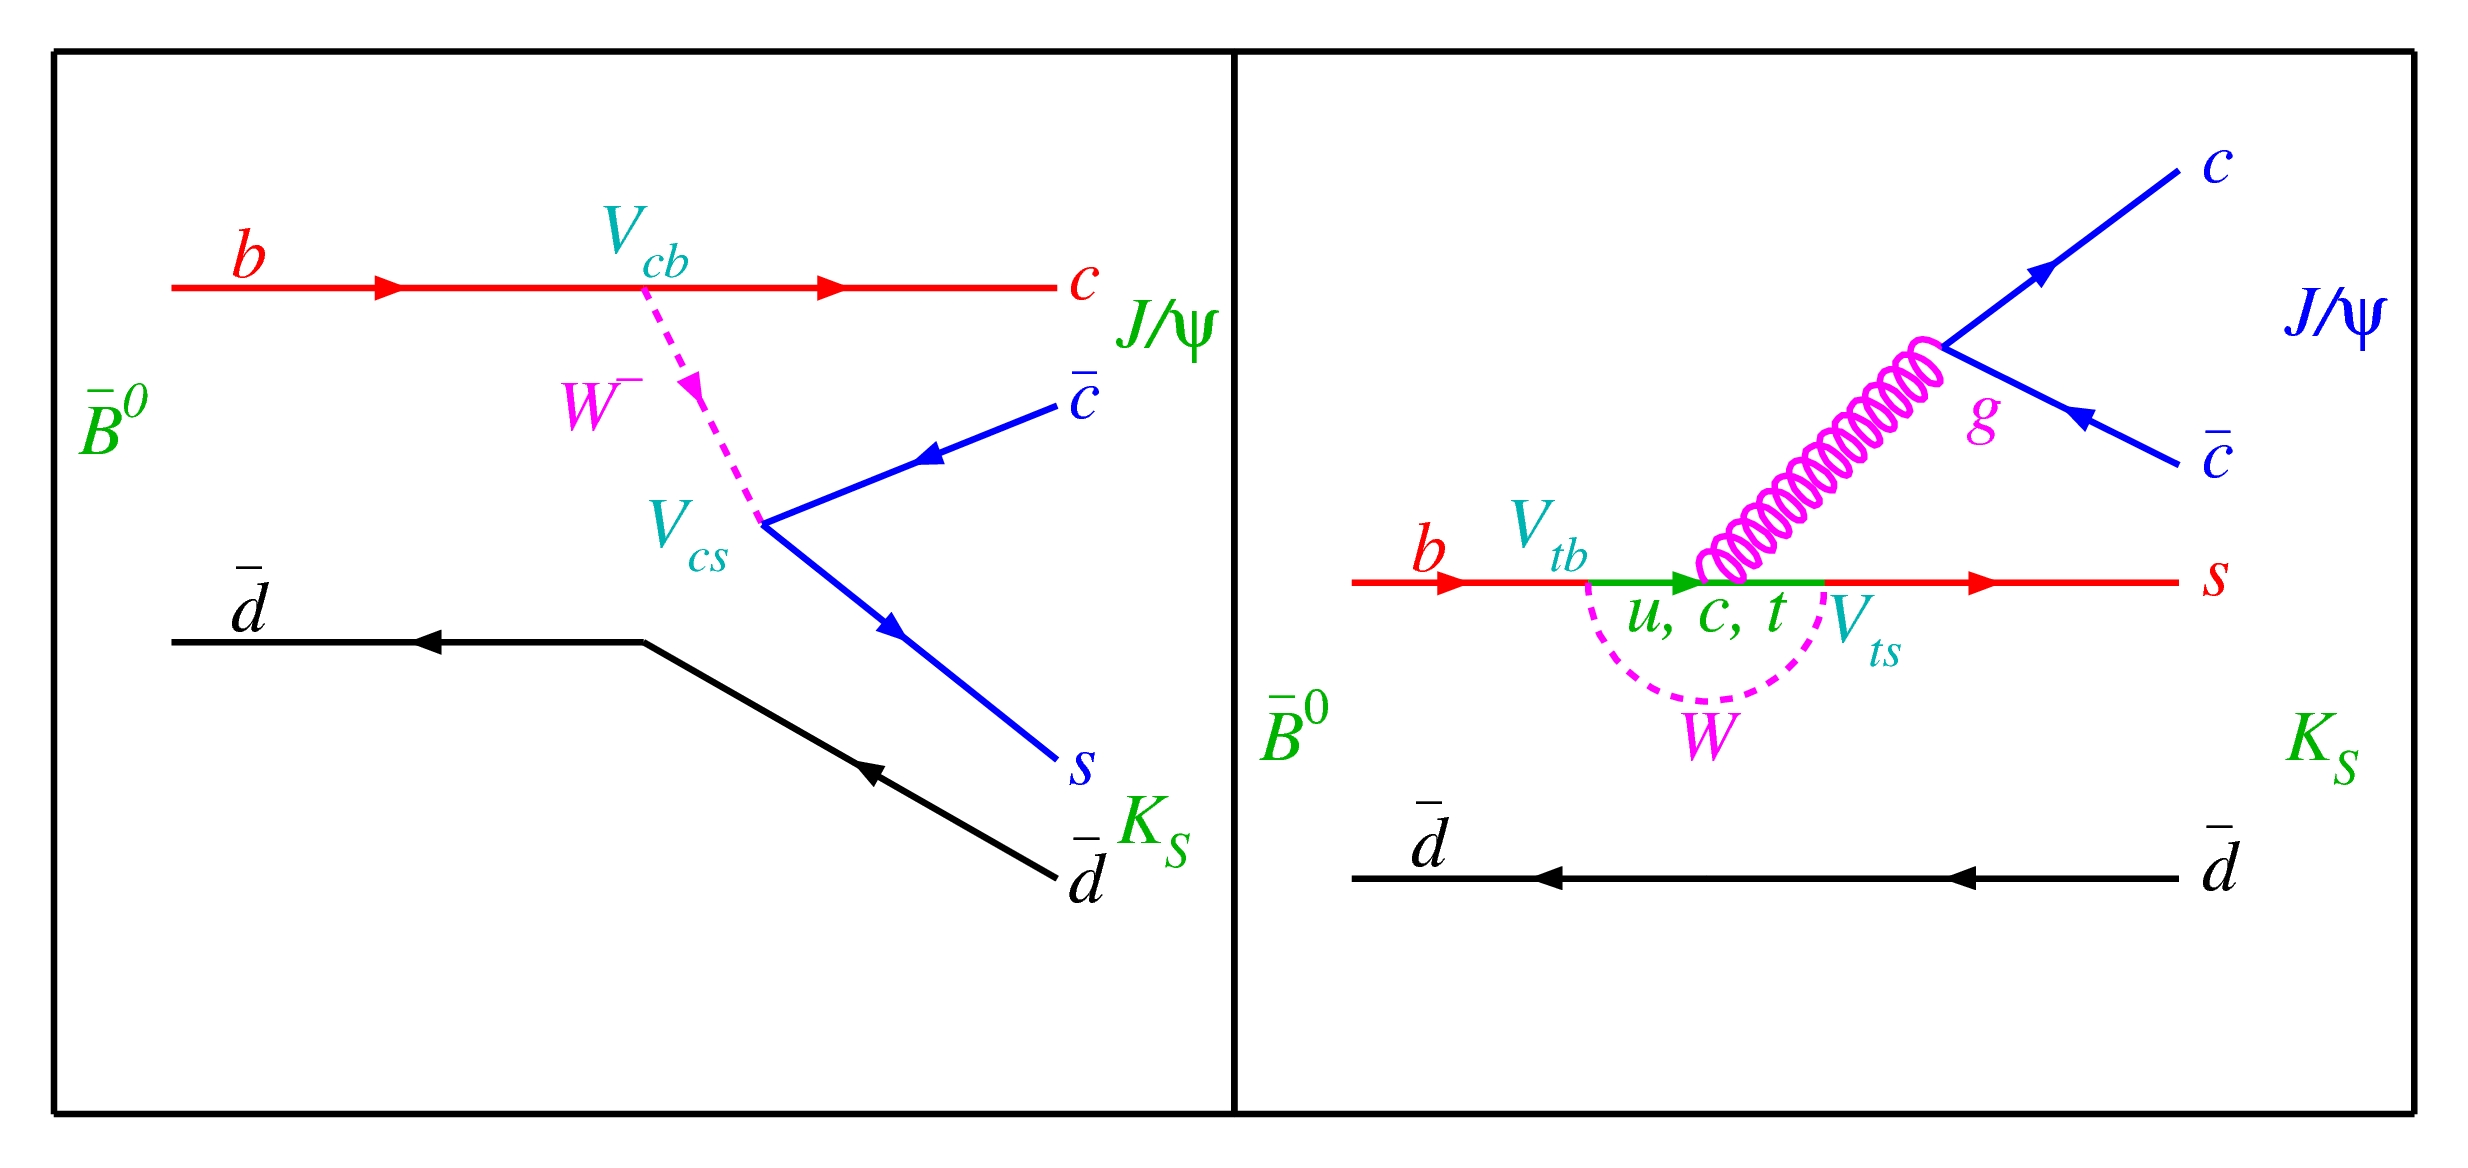
\includegraphics[width=\textwidth]{bd2jpsikshort}
\caption{Feynmangraph zum Zerfall \Decaychannel. Links: Baumdiagramm, rechts: Pinguindiagramm}
\label{fig:decay}
\end{figure}

\section{Diskrete Symmetrietransformationen}
Symmetrien sind in der Physik von zentraler Bedeutung. Gemäß dem Noether-Theorem existiert in der klassischen Physik zu jeder kontinuierlichen Symmetrie eine Erhaltungsgröße. In quantenmechanischen Systemen können wir drei diskrete Symmetrietransformationen betrachten:
\begin{enumerate}
\item \textbf{Parität $\mathcal{P}$:} \\
      Bei der Paritätsoperation wird das Vorzeichen der kartesischen Ortskoordinaten umgekehrt. Dies entspricht einer Punktspigelung.
\item \textbf{Ladungskonjugation $\mathcal{C}$:} \\
      Jedes Teilchen wird durch sein Antiteilchen ersetzt.
\item \textbf{Zeitumkehr $\mathcal{T}$:} \\
      Das Vorzeichen auf der Zeitachse wird umgekehrt. Da in der vorligenden Arbeit allerdings nur die CP-Verletzung gemessen werden soll, wird die Zeitumkehr im folgenden vernachlässigt.
\end{enumerate}
Entgegen der klassischen Intuition konnte Wu 1956 nachweisen, dass die Parität im $\beta$-Zerfall und damit in der schwachen Wechselwirkung nicht erhalten ist. Weitere Experimente zeigen, dass die schwache Wechselwirkung die Parität maximal verletzt: Neutrinos, die nur schwach wechselwirken können, sind stets \glqq linkshändig\grqq (Spin und Impuls antiparallel), Antineutrinos dagegen immer \glqq rechtshändig\grqq (Spin und Impuls parallel). Da der Spin im Gegensatz zum Impuls invariant unter $\mathcal{P}$-Transformation ist, würde diese Operation aus einem linkshändigen Neutrino ein rechtshändiges machen, was in der Nautr nicht realisiert ist.

Damit ist offensichtlich, dass die schwache Wechselwirkung auch die Ladungskonjugation verletzt: Wendet man die $\mathcal{C}$-Transformation auf ein linkshändiges Neutrino an, so erhält man ein linkshändiges Antineutrino. Dieses existiert aber wie bereits erwähnt nicht. Analog gilt die Überlegung auch für Antineutrinos.

\subsection{Scheinbare $\mathcal{CP}$-Invarianz}
Wendet man nun aber die Transformationen $\mathcal{P}$ und $\mathcal{C}$ direkt hintereinander an, so ergibt sich zunächst kein Widerspruch zur Natur (siehe Abb. \ref{fig:cp_invarianz}). Aus einen linkshändigen Neutrino wird ein rechtshändiges Antineutrino. Im Jahre 1964 wurde dann allerdings im Zerfall neutraler K-Mesonen erstmals $\mathcal{CP}$-Verletzung nachgewiesen. \cite{kleinknecht}

\begin{figure}[hptb]
\centering
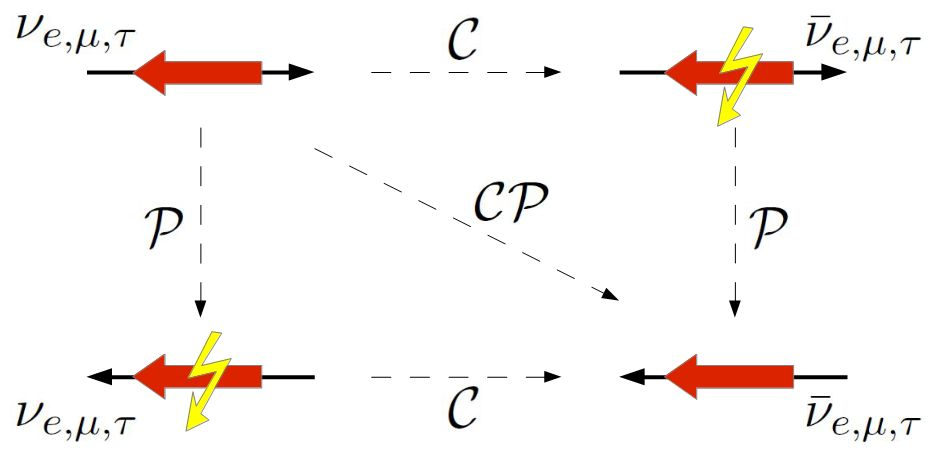
\includegraphics[width = 0.8\textwidth]{cp_invarianz}
\caption{Scheinbare $\mathcal{CP}$-Invarianz: Während eine reine $\mathcal{P}$- oder $\mathcal{C}$-Transformation zu in der Natur nicht realisierten Zuständen führt, scheint es bei der kombinierten $\mathcal{CP}$-Transformation keinen Widerspruch zu geben (dünne Pfeile: Impulsausrichtung, dicke Pfeile: Spinausrichtung).}
\label{fig:cp_invarianz}
\end{figure}



\section{\CP-Verletzung in der Mischung}
Die Flavoureigenzustände $\Ket{B^0} = \Ket{\overline{b}d}$ und $\Ket{\overline{B^0}} = \Ket{b\overline{d}}$ entsprechen nicht den Masseneigenzuständen. Wir definieren daher die normierten Zustände
\begin{align}
\Ket{B_h} = p \Ket{B^0} - q \Ket{\overline{B^0}} \label{eq:b_heavy}\\ 
\Ket{B_l} = p \Ket{B^0} + q \Ket{\overline{B^0}} \label{eq:b_light}\\
\text{mit} \quad |p|^2 + |q|^2 = 1
\end{align}
welche eine definierte Masse und Zerfallsbreite besitzen. Sie sind auch Eigenzustände eines nicht-hermiteschen Hamiltonoperators (Nichthermitizität wegen des möglichen Zerfalls der Teilchens). Dieser setzt sich zusammen aus den hermiteschen Massenoperatoren $M$ und $\Gamma$. Notieren wir die lineare Superposition der Zustände \ref{eq:b_heavy} und \ref{eq:b_light} als $\begin{pmatrix} p \\ q \end{pmatrix}$, so nimmt die zeitabhängige Schrödingergleichung die Form
\begin{align}
\im \diff{}{t}\begin{pmatrix} p \\ q \end{pmatrix} = \left(M - \frac{\im}{2} \Gamma\right) \begin{pmatrix} p \\ q \end{pmatrix}
\end{align}
an und führt zur folgenden zeitlichen Entwicklung der Zustände:
\begin{align}
\nonumber \Ket{B_{h/l}(t)} &= \e^{-\im m_{h/l}t-\frac{1}{2}\Gamma_{h/l}t}\Ket{B_{h/l}(0)} \\
                           &= \e^{-\gamma_{h/l}t}(p\Ket{B^0} \mp q\Ket{\overline{B^0}}) \\
&\text{mit} \quad \gamma_{h/l} = \im m_{h/l}+\frac{\Gamma_{h/l}}{2}
\end{align}
Hierbei ist $\gamma_{h/l}$ so definiert, dass $-\im\gamma_{h/l} = m_{h/l}-\frac{\im}{2}\Gamma_{h/l}$ die Eigenwerte des Hamiltonoperators $\mathcal{H} := \left(M - \frac{\im}{2} \Gamma\right)$ sind. Umgeschrieben auf die Flavoureigenzustände erhält man:
\begin{align}
\nonumber \Ket{B^0(t)} &= \frac{1}{2p}\left(\Ket{B_h} + \Ket{B_l}\right) \\
                       &= \frac{1}{2}\left[ (\e^{-\gamma_h t}+\e^{-\gamma_l t})\Ket{B^0} - \frac{q}{p}(\e^{-\gamma_h t}-\e^{-\gamma_l t})\Ket{\overline{B^0}}\right] \label{eg:b(t)}
\end{align}
Die Wahrscheinlichkeit für den Übergang eines $\Ket{B^0}$ (zum Zeitpunkt $t=0$) in ein $\Ket{\overline{B^0}}$ beträgt:
\begin{align}
\nonumber P(B^0\rightarrow\overline{B^0})(t) &= |\Braket{\overline{B^0}|B^0(t)}|^2 \\
                                        &= \frac{1}{4} \left|\frac{q}{p}\right|^2 \left[\e^{-\Gamma_h t} + \e^{-\Gamma_l t} - 2\e^{-\frac{1}{2}(\Gamma_h + \Gamma_l) t}\cos(\Delta m_d t)\right] \\
&\text{mit} \quad \Delta m_d = m_h - m_l
\end{align}

Analog gilt für die Übergangswahrscheinlichkeit eines $\Ket{\overline{B^0}}$ in ein $\Ket{B^0}$:
\begin{align}
P(\overline{B^0}\rightarrow B^0)(t) = \frac{1}{4} \left|\frac{p}{q}\right|^2 \left[\e^{-\Gamma_h t} + \e^{-\Gamma_l t} - 2\e^{-\frac{1}{2}(\Gamma_h + \Gamma_l) t}\cos(\Delta m_d t)\right] 
\end{align}

Es kommt daher in der Mischung zur \CP-Verletzung, wenn die Oszillation ungleichmäßig verläuft, anders ausgedrückt:
\begin{align}
\text{\CP-Verletzung in der Mischung} \qquad \Longleftrightarrow \qquad \left|\frac{p}{q}\right| \neq 1 
\end{align}

\section{Direkte \CP-Verletzung}
Die Zerfallsamplituden der neutralen $B^0$-Mesonen in einen Endzustand $\Ket{f}$ bzw. seinen \CP-konjugierten Zustand $\Ket{\overline{f}}$ sind definiert als
\begin{alignat}{2}
\nonumber A_f &= \Braket{f|\mathcal{H}|B^0}, && \qquad A_{\overline{f}} = \Braket{\overline{f}|\mathcal{H}|B^0}, \\
          \overline{A_f} &= \Braket{f|\mathcal{H}|\overline{B^0}}, && \qquad  \overline{A_{\overline{f}}} = \Braket{\overline{f}|\mathcal{H}|\overline{B^0}}. \label{eq:decay_amplitudes}
\end{alignat}
Dabei bezeichnet $\mathcal{H}$ einen Hamiltonoperator der schwachen Wechselwirkung. Ist \CP erhalten, dann sollten die Zerfallsraten, ergo auch die Zerfallsamplituden eines $B^0$ nach $f$ sowie eines $\overline{B^0}$ nach $\overline{f}$ gleich sein. Dies bedeutet:
\begin{align}
\text{Direkte \CP-Verletzung} \qquad \Longleftrightarrow \qquad \frac{|A_f|}{|\overline{A_{\overline{f}}}|} \neq 1 \quad \text{bzw.} \quad \frac{|\overline{A_f}|}{|A_{\overline{f}}|} \neq 1
\end{align}


\section{\CP-Verletzung in der Interferenz}
Die Zustände \ref{eq:b_heavy} und \ref{eq:b_light} haben eine nahezu gleiche Anzahl an Zerfällskanäle. Dies hat zur Folge, dass die Lebensdauern des schweren und leichten Zustands innerhalb weniger Prozent gleich sind:
\begin{align}
\Gamma := \Gamma_h = \Gamma_l \label{eq:Gamma}
\end{align}

Weiterhin sagt das Standard Modell nur eine kleine \CP-Verletzung in der \Bd - \Bdbar - Mischung voraus, sodass
\begin{align}
\left|\frac{p}{q}\right| = 1 \qquad \text{in} \mathcal{O}(10^{-3}). \label{eg:pq_approx}
\end{align}

Für das B-Meson-System bleibt daher nur die Möglichkeit der \CP-Verletzung in der Interferenz von Mischung und direktem Zerfall. Der in dieser Arbeit betrachtete Zerfallskanal $B_d^0 \rightarrow J/\Psi K_s^0$ hat einen \CP-Eigenzustand als Endzustand (\CP $\Ket{\JPsi\Kshort} = -\Ket{\JPsi\Kshort}$). In Anlehnung an \ref{eq:decay_amplitudes} sind die Zerfallsamplituden hier definiert als
\begin{align}
\nonumber A_f := \Braket{f|B^0(t)}, \qquad \overline{A_{f}} := \Braket{f|\mathcal{H}|\overline{B^0}}
\end{align}

Mit Blick auf die Zerfallsamplituden der Masseneigenzustände wird die komplexe Größe
\begin{align}
\lambda_f := \frac{q\overline{A_f}}{pA_f} \label{eq:lambda}
\end{align}
definiert. Ausgehend von Gleichung \ref{eg:b(t)} sowie mit Hilfe fer Gleichungen (\ref{eq:Gamma}), (\ref{eg:pq_approx}) und (\ref{eq:lambda}) gilt für die Zerfallsrate eines anfänglich reinen \Bd-Zustands:
\begin{align}
\nonumber \Gamma (B^0 \rightarrow \JPsi\Kshort) &= \frac{1}{4}\left| (\e^{-\gamma_h t}+\e^{-\gamma_l t})A_f - \frac{q}{p}(\e^{-\gamma_h t}-\e^{-\gamma_l t})\overline{A_f}\right|^2 \\
&= \frac{1}{2} \left|A_f\right|^2\e^{-\Gamma t} \left[1+|\lambda_f|^2 + (1-|\lambda_f|^2)\cos(\Delta m_d t) - 2\mathrm{Im}(\lambda_f)\sin(\Delta m_d t)\right]
\end{align}
Analog:
\begin{align}
\Gamma (\overline{B^0} \rightarrow \JPsi\Kshort) &= \frac{1}{2} \left|A_f\right|^2\e^{-\Gamma t} \left[1+|\lambda_f|^2 -(1-|\lambda_f|^2)\cos(\Delta m_d t) + 2\mathrm{Im}(\lambda_f)\sin(\Delta m_d t)\right]
\end{align}

Damit kann die vom Standard Modell prognostizierte \CP-verletzende Asymmetrie 
\begin{align}
\mathcal{A}_{\text{\CP}} &= \frac{\Gamma (\overline{B^0} \rightarrow \JPsi\Kshort) - \Gamma (B^0 \rightarrow \JPsi\Kshort)}{\Gamma (\overline{B^0} \rightarrow \JPsi\Kshort) + \Gamma (B^0 \rightarrow \JPsi\Kshort)} \\
&= -\frac{1-|\lambda_f|^2}{1+|\lambda_f|^2}\cos(\Delta m_d t) + \frac{2\mathrm{Im}(\lambda_f)}{1+|\lambda_f|^2}\sin(\Delta m_d t) \\
&=: \CJPsi \cos(\Delta m_d t) + \SJPsi \sin(\Delta m_d t)
\end{align}
berechnet werden und vereinfacht sich - da $\Ket{\JPsi\Kshort}$ ein \CP-Eigenzustand ist, gilt $|\lambda_f| = 1$ - hier zu
\begin{align}
\mathcal{A}_{\text{\CP}} = \mathrm{Im}(\lambda_f)\sin(\Delta m_d t) .
\end{align}

Damit kann im B-Meson-System, insbesondere im Zerfall $B_d^0 \rightarrow J/\Psi K_s^0$ durch Messung der Asymmetrie-Amplitude $\SJPsi$ \CP-Verletzung in der Interferenz gemessen werden.

\begin{align}
\text{\CP-Verletzung in der Interferenz} \qquad \Longleftrightarrow \qquad \SJPsi = \mathrm{Im}(\lambda)\neq 0
\end{align}

\section{CKM-Formalismus}
Durch Austausch eines W$^{\pm}$-Bosons können Quarks ihren Flavour ändern. Dabei sind sie aber nicht an ihre jeweilige Generation gebunden, sondern können - wenn auch zum Teil stark unterdrückt - prinzipiell den Flavour einer jeden Generation annehmen. Ein kleines Beispiel: Der Eigenzustand $\Ket{u}$ der starken Wechselwirkung geht über den schwachen Prozess (Austausch eines W$^{\pm}$-Bosons) nicht in ein $\Ket{d}$ über, sondern vielmehr in eine Linearkombination aus $\Ket{d}$, $\Ket{s}$ und $\Ket{b}$, die im folgenden mit $\Ket{d'}$ bezeichnet wird. Allgemein werden die möglichen Linearkombinationen durch die Cabibbo-Kobayashi-Maskawa-Matrix (kurz: CKM-Matrix) beschrieben.
\begin{align}
\begin{pmatrix}
\Ket{d'} \\ \Ket{s'} \\ \Ket{b'}
\end{pmatrix}
=
\begin{pmatrix}
V_{ud} & V_{us} & V_{ub} \\
V_{cd} & V_{cs} & V_{cb} \\
V_{td} & V_{ts} & V_{tb} \\
\end{pmatrix}
\cdot
\begin{pmatrix}
\Ket{d} \\ \Ket{s} \\ \Ket{b}
\end{pmatrix}
\end{align}

Das Betragsquadrat eines jeden Matrixelementes $|V_{ij}|^2$ gibt dabei die Wahrscheinlichkeit für den Übergang eines Quarks $\Ket{i}$ in ein $\Ket{j}$ an. Da die $V_{ij}$ prinzipiell komplex sein können, gibt es zunächst 18 freie Parameter, die zu bestimmen sind. Diese Zahl reduziert sich zum einen um 5 relative Quarkphasen, die physikalisch nicht beobachtbar sind. Zum anderen reduziert die Forderung nach Unitarität der CKM-Matrix die Zahl der unabhängigen Parameter um 9, sodass am Ende 4 Parameter, 3 Euler Winkel sowie eine Phase, welche für die \CP-Verletzung verantwortlich ist, zu bestimmen sind. Die CKM-Matrix lässt sich näherungsweise durch die Wolfenstein-Parametrisierung darstellen:

\begin{align}
V_{\text{CKM}}=
\begin{pmatrix}
V_{ud} & V_{us} & V_{ub} \\
V_{cd} & V_{cs} & V_{cb} \\
V_{td} & V_{ts} & V_{tb} \\
\end{pmatrix}
=
\begin{pmatrix}
1-\frac{\lambda^2}{2} & \lambda & A\lambda^3(\rho-\im\eta) \\
-\lambda & 1-\frac{\lambda^2}{2} & A\lambda^2 \\
A\lambda^3(1-\rho-\im\eta) & -A\lambda^2 & 1
\end{pmatrix}
+ \mathcal{O}(\lambda^4)
\end{align}

Für den Zerfall von \Bd-Mesonen ist die Unitaritätsbedingung
\begin{align}
V_{ud}V_{ub}^* + V_{cd}V_{cb}^* + V_{td}V_{tb}^* = 0
\end{align}
von besonderer Bedeutung. Man kann die einzelnen Summanden nun in der $(\rho,\eta)$-Ebene auftragen und erhält dabei ein sogenanntes Unitaritätsdreieck. Es wird so normiert, dass die Unterseite bei (0,0) beginnt und bei (1,0) endet (siehe Abb. \ref{fig:unitarity}). Die obere Ecke liegt dann bei $(\overline{\rho}, \overline{\eta})$, wobei $\overline{\rho} = \rho(1-\lambda^2/2)$ und $\overline{\eta} = \eta(1-\lambda^2/2)$ gemäß der Wolfenstein-Parametrisierung sind. Die Winkel des Dreiecks erhält man über
\begin{align}
\alpha = \text{arg}\left[-\frac{V_{td}V_{tb}^*}{V_{ud}V_{ub}^*}\right], \qquad
\beta = \text{arg}\left[-\frac{V_{cd}V_{cb}^*}{V_{td}V_{tb}^*}\right], \qquad
\gamma = \text{arg}\left[-\frac{V_{ud}V_{ub}^*}{V_{cd}V_{cb}^*}\right].
\end{align}

\begin{figure}[hptb]
\centering
%\includegraphics[width=\textwidth]{•}
\caption{Unitaritätsdreieck}
\label{fig:unitarity}
\end{figure}

Das Standardmodell stellt für den hier untersuchten Zerfallskanal eine Beziehung zwischen dem Winkel $\beta$ und der komplexen Größe $lambda_f$ aus Gleichung \ref{eq:lambda} her (\cite{nir}, \cite{noguchi}):
\begin{align}
&\lambda_f = \underbrace{\frac{V_{td}V_{tb}^*}{V_{td}^*V_{tb}}}_{\frac{q}{p}} \underbrace{\frac{V_{cd}^*V_{cb}}{V_{cd}V_{cb}^*}}_{\frac{\overline{A_f}}{A_f}} = \e^{2\im\beta} \\
\Longrightarrow &\SJPsi = \mathrm{Im}(\lambda_f) = \sin(2\beta).
\end{align}
 
Durch Messung der Amplitude der \CP-Asymmetrie kann man direkte Rückschlüsse auf den CKM-Winkel $\beta$ ziehen.

\chapter{Abschätzung systematischer Fehler}
\section{Tagging Kalibrierung}
Im Fit wird bei den Parametern der Tagging Kalibrierung nur der statistischen Fehler berücksichtigt. Es soll nun an dieser Stelle der Einfluss der statistischen Unsicherheiten abgeschätzt werden. \\
Die Korrekturparameter $p_0$ und $p_1$ für die Fehlerwahrscheinlichkeit des \gls{OST} sind gegeben durch
\begin{align}
p_0 &= 0,392 \pm 0,0017\ \text{(stat.)} \pm 0,0076\ \text{(syst.)} \\
p_1 &= 1,035 \pm 0,021\ \text{(stat.)} \pm 0,0076\ \text{(syst.)}.
\end{align}

\paragraph{Variation der Parameter in den Daten}
Zunächst werden die Startwerte der Parameter $p_0$ und $p_1$ variiert, indem man jeweils den systematischen Fehler der Parameter addiert bzw. subtrahiert und dann den Fit auf die Daten durchührt. Für alle vier Kombinationen wird dann die Abweichung vom regulären Fitergebnis für $\SJPsi$ berechnet. Der Referenzwert aus dem Fit beträgt
\begin{align}
\SJPsi = 0,625 \pm 0,069
\end{align}

\begin{table}[hptb]
\centering
\caption{Variation des Fitergebnisses für $\SJPsi$ bei Veränderung der Startwerte für $p_0$ und $p_1$ $\pm$ ihrer statistischen Unsicherheiten}
\label{tab:syst_fit_calib_data}
$\begin{array}{cc|c|c}
\hline\hline
p_0            & p_1           & \SJPsi          & \Delta\SJPsi   \\ \hline
0,392 - 0,0076 & 1,035 - 0,012 & 0,599 \pm 0,067 & -0,026 \pm xxx \\
0,392 + 0,0076 & 1,035 - 0,012 & 0,661 \pm 0,072 & 0,036 \pm xxx \\
0,392 - 0,0076 & 1,035 + 0,012 & 0,592 \pm 0,066 & -0,033 \pm xxx \\
0,392 + 0,0076 & 1,035 + 0,012 & 0,651 \pm 0,071 & 0,026 \pm xxx \\
\hline\hline
\end{array}$
\end{table}

Die Ergebnisse sind Tabelle \ref{tab:syst_fit_calib_data} zu entnehmen. Die größte Abweichung beträgt hier $\Delta\SJPsi = 0,036$.

\paragraph{Variation der Parameter in \gls{Toy MC}}
Eine weitere Möglichkeit der Abschätzung besteht darin, sich entsprechende Toys zu generieren und diese dann zu fitten. Im Folgenden werden bei der Toy Generierung die Parameter $p_0$ und $p_1$ um ihre systematische Unsicherheiten variiert, der Fit dann allerdings mit den ursprünglichen Parameterwerten durchgeführt. Als Referenzwert generieren und fitten wir toys mit den ursprünglichen Parameterwerten $p_0$ und $p_1$ sowie $\SJPsi = 0.75$ und erhalten hierfür:

\begin{align}
\SJPsi = 0,75527 \pm xxx
\end{align}

\begin{table}[hptb]
\centering
\caption{Variation des Fitergebnisses für $\SJPsi$ bei Veränderung der Parameterwerte $p_0$ und $p_1$ $\pm$ ihrer statistischen Unsicherheiten bei der Generierung von Toys}
\label{tab:syst_fit_calib_toys}
$\begin{array}{cc|c|c}
\hline\hline
p_0            & p_1           & \SJPsi          & \Delta\SJPsi   \\ \hline
0,392 - 0,0076 & 1,035 - 0,012 & 0,782 \pm xxx & 0,027 \pm xxx \\
0,392 + 0,0076 & 1,035 - 0,012 & 0,719 \pm xxx & -0,036 \pm xxx \\
0,392 - 0,0076 & 1,035 + 0,012 & 0,788 \pm xxx & 0,032 \pm xxx \\
0,392 + 0,0076 & 1,035 + 0,012 & 0,727 \pm xxx & -0,028 \pm xxx \\
\hline\hline
\end{array}$
\end{table}

Die Ergebnisse sind Tabelle \ref{tab:syst_fit_calib_toys} zu entnehmen. Die größte Abweichung beträgt hier betragsmäßig ebenfalls $\Delta\SJPsi = 0,036$. Daher schätzen wir den systematischen Fehler durch die Tagging Kalibrierung auf 

\begin{align}
s_{tag_calib} = 0.036 \ .
\end{align}

\begin{thebibliography}{---}
\bibitem{kleinknecht}  K. Kleinknecht, Uncovering ...
\end{thebibliography}

\printglossaries 
% Selbstständigkeitserklärung
\chapter*{Erklärung}

Ich versichere, dass ich diese Arbeit selbstständig verfasst und keine anderen als die angegebenen Quellen und Hilfsmittel benutzt habe. \\
\vspace{0.2cm}
\begin{flushleft}
Heidelberg, den 19.08.2013,\\
\vspace{2cm}
%Unterschrift
Patrick Fahner
\end{flushleft}


\end{document}


